\section{Estrutura da Base de Recarga} % (fold)
\label{sec:estrutura_da_base}
	
	Uma base fixa é responsável por realizar a recarga do robô, além do carregador da bateria estará nessa estrutura a Raspberry Pi.

	\subsection{Solução} % (fold)
	\label{sub:solução}
		
		A base precisa armazenar o Raspberry Pi, o carregador do aspirador, o roteador Wireless e a fonte de energia para o Raspberry Pi. Para tal tarefa, a base terá uma carcaça retangular de dimensões 250x250x200mm. O material usado será o acrílico ou PVC pelos mesmos motivos explicitados anteriormente na seção da estrutura. 

		Para realizar o encaixe do carregador a estrutura do robô será usado um conector do tipo magnético, pois esse tipo de conector garante um encaixe mais preciso entre os conectores.

		\begin{figure}[H]
			\centering
			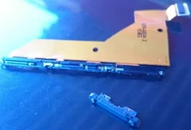
\includegraphics[scale=0.8]{figuras/conector_mag.png}
			\caption{Conectores magnético modelo Sony Xperia.}
			\label{img:conectores}
		\end{figure}

		\begin{figure}[H]
			\centering
			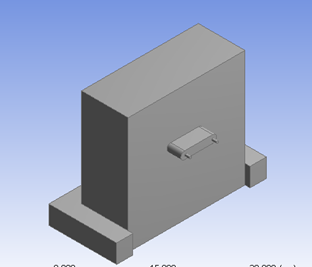
\includegraphics[scale=0.8]{figuras/estrutura_base.png}
			\caption{Estrutura da base de recarga.}
			\label{img:estrutura_base}
		\end{figure}	
	

	% subsection solução (end)
% section estrutura_da_base (end)